\documentclass[12pt,a4paper, titlepage]{article}
\usepackage{amsmath}
\usepackage{graphicx}
\usepackage{float}
\usepackage{wrapfig}
\usepackage[russian]{babel}
\usepackage[utf8]{inputenc}


\title{Оценка кривизны для неструктурированных триангуляций поверхностей}
\date{2021\\Май}
\author{Петраков Иван\\\ МФТИ\\\\\\\\\\\\\\\\\\\\}
\hoffset = 0pt
\voffset = 0pt
\textheight = 700pt
\topmargin = 0pt
\headheight = 0pt
\headsep = 0pt
\marginparwidth = 0pt
\oddsidemargin = 0pt
\textwidth = 450pt

\begin{document}

\maketitle

\subsection*{Введение}
\noindent\rule{\textwidth}{1pt}
Знание кривизны поверхностей необходимо, например, в симуляции потока, компьютерной графике и анимациях. Отдельное внимание заслуживает работа с изменяющейся геометрией. Таке применения, в основном, не имеют гладкой аналитической формы поверхности, формирующей модельную геометрию. Наоборот, они работают с большим количеством дискретной информации, соединяющей точки на поверхности с формой неструктурированной сетки. Поэтому очень важно правильно оценивать локальную кривизну точек на таких дискретных поверхностях.
\\
\\
В этой работе будут приведены два различных подхода к решению поставленной задачи - оценке кривизны для неструктурированной триангуляции поверхности. Первый подход основан на дискретной дифференциальной геометрии, второй же основан на подгонке квадриков. В каждом разделе сначала будут описываться методы, затем будут приведены модели, на которых будет основываться тест сходимости, после чего будут обсуждены результаты тестов. Напоследок, будут представлены результаты на больших сетках.

\subsection*{Оценка кривизны с использованием дискретной дифференциальной геометрии}
\noindent\rule{\textwidth}{1pt}
Этот метод основан на пространственном усреднении триангуляционной информации с использованием дискретной дифференциальной геометрии. Гауссова кривизна оценивается как дискретная форма теоремы Гаусса-Бонета, примененная к 1-кольцевой окрестности вершины. Оценка для средней кривизны выводится из дискретизации оператора Лапласа-Бельтрами, который также применяется на 1-кольцевой окрестности. Предположим, что у нас дан некоторый набор треугольников, окружающих точку $x_i$ (см. рисунок 1), тогда оценка для Гауссовой кривизны $K_i$ и средней кривизны $H_i$ в заданной точке определяются как

\begin{equation}
\begin{cases}
K_i = \frac{1}{A}(2 \pi - \sum_j{\theta_j})
\\
2 H_i \vec{n_i} = \frac{1}{2 A} \sum_j{(cot \alpha_{ij} + cot \beta_{ij})}(x_i - x_j)
\end{cases}
\end{equation}

Здесь А - площадь некоторой области вокруг заданной точки, $\vec{n_i}$ - вектор нормали к заданной точки, $x_j, \theta_j, \alpha_{ij}, \beta_{ij}$ показаны на рисунке.
\\
\\
Доказано, что ошибка вычисления кривизны минимальна тогда, когда А - область (диаграмма) Вороного, определяющаяся как "берем центры сторон треугольников, проходящих через заданную точку, проводим через них нормальные прямые, полученная пересечением всех прямых область и есть область Вороного". Площадь области Вороного определяется как
\begin{equation}
A_{vor} = \frac{1}{8}\sum_j{(cot \alpha_{ij} + cot \beta_{ij})}||x_i - x_j||^2
\end{equation}
\\
\\
В случае получения тупоугольных треугольников предлагается проводить нормальную прямую через сторону, противоположную тупому углу, но ошибка получается выше. Стоит также отметить, что минимизация ошибки при использовании области Вороного не доказана на результатах сходимости.

\begin{figure}[H]
	\centering
	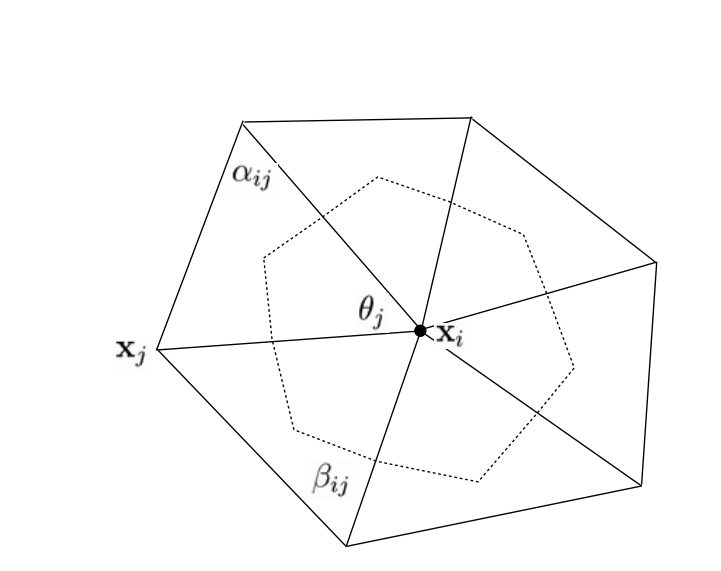
\includegraphics[width = 0.8\textwidth]{1.png}
\end{figure}


\subsection*{Оценка кривизны с использованием подгонки квадриков}
\noindent\rule{\textwidth}{1pt}
Методы подгонки квадриков основаны на идее, что гладкая поверхность может быть локально аппроксимирована квадратично полиномиальной поверхностью. Таким образом, методы стараются приблизить квадрики к точкам в локальной окрестности каждой точки интереса. Приведем пошаговый алгоритм подгонки квадрика формы $Z' = a X'^2 + b X' Y' + c Y'^2$.
\\
\\
1. Оцениваем нормаль $\vec{n}$ к поверхности в точке $\vec{p}$ интереса. Это можно сделать несколькими способами (усреднением соседствующих триангуляционных нормалей, методом наименьших квадратов).
\\
\\
2. Строим в точке интереса локальную систему координат ($X', Y', Z'$), где $Z'$ направлена по приближенной нормали. Для исправления первой координаты предлагается выровнять $X'$ по проекции глобальной оси $X$ на касательную плоскость, определяемую приближенной нормалью. В результате получается матрица поворота от глобальной координатной сетки к локальной. $\vec{R} = [\vec{r_1}, \vec{r_2}, \vec{r_3}]^{T}$. Здесь 
\begin{equation}
\begin{cases}
\vec{r_3} = \vec{n}
\\
\vec{r_1} = \frac{I - \vec{n}\vec{n}^T}{||I - \vec{n}\vec{n}^T||} \vec{i}
\\
\vec{r_2} = \vec{r_3} \times \vec{r_1}
\end{cases}
\end{equation}
Здесь $I$ - тождественная матрица, $\vec{i}$ - глобальная ось X.
\\
\\
Осталось обсудить ситуацию, когда при при вычислении получается нулевой вектор. В таком случае необходимо взять проекцию на какую-нибудь другую глобальную ось.
\\
\\
3. Выбираем набор точек, используемых для приближения квадрика. Самым простым выбором оказывается соседи рассматриваемого узла, связанные по краям.
\\
\\
4. Переводим координаты выбранных точек из глобальной в локальную систему координат по $\vec{x'} = \vec{R}(\vec{x} - \vec{p})$.
\\
\\
5. Вычисляем коэффициенты квадрика методом наименьших квардратов для системы
\begin{equation}
\begin{cases}
a x_1^2 + b x_1 y_1 + c y_1^2 = z_1
\\
...
\\
a x_n^2 + b x_n y_n + c y_n^2 = z_n
\end{cases}
\end{equation}
\\
\\
6. Оцениваем основные кривизны, $\kappa_1$ и $\kappa_2$, Гауссову кривизну $K$ и среднюю кривизну $H$ (все в точке $\vec{p}$) как
\begin{equation}
\begin{cases}
\kappa_1 = a + c + \sqrt{(a-c)^2 + b^2}
\\
\kappa_2 = a + c - \sqrt{(a-c)^2 + b^2}
\\
K = 4 a c - b^2
\\
H = a + c
\end{cases}
\end{equation}
\\
\\
Оценка кривизны с использованием такого (простого) квадрика достаточно чувствительна к оценке нормали к поверхности. Расширенная подгонка квадрика старается уменьшить эту чувствительность вводя линейные члены в приближенный квадрик, то есть теперь он задается как $Z' = a X'^2 + b X' Y' + c Y'^2 + d X' + e Y'$. Коэффициенты такого квадрика могут быть использованы для вычисления новой оценки нормали поверхности как
\begin{equation}
\vec{n} = \frac{1}{\sqrt{d^2+e^2 + 1}} [-d, e, 1]^T
\end{equation}
\\
\\
Повторяя шаги 1-5, приводим к исправленным формулам
\begin{equation}
\begin{cases}
K = \frac{4 a c - b^2}{(1+d^2+e^2)^2}
\\
H = \frac{a + c + ae^2 + cd^2 - b d e}{(1+d^2+e^2)^{3/2}}
\end{cases}
\end{equation}
\\
Проблема расширенного метода заключается в том, что для его построения необходимо как минимум 5 точек вместо 3, как в простом методе. Существует исправление (улучшение) этой проблемы, однако в обзорной презентации не считаю необходимым останавливаться на этом.
\subsection*{Тесты сходимости}
\noindent\rule{\textwidth}{1pt}
Возьмем шестиугольник из треугольников радиуса $L$, вершины которого $\vec{x_i}$, $i = 1, 6$ и центр $\vec{p}$ находятся на цилиндрической поверхности фиксированного радиуса $r < L$. Предположим, что ось цилиндра совпадает с осью $Z$, а ось $X$ проходит через вершину. Тогда $\vec{p} = [r, 0, 0]^T$. Координаты $\vec{x_2}$ и $\vec{x_5}$ равны соответственно $[r, 0, -L]^T$ и $[r, 0, L]^T$.
\\
Если координаты внешнего узла шестиугольника заданы как $[x_i, y_i, z_i]^T$, тогда выполняются следующие соотношения
\begin{equation}
\begin{cases}
x_i^2 + y_i^2 = r^2
\\
(x_i - r)^2 + y_i^2 + z_i^2 = L^2
\end{cases}
\end{equation}
Взяв $z_i = \pm L/k$, получаем
\begin{equation}
x_i = \frac{1}{2r}(r^2 - L^2(1 - \frac{1}{k^2})
\end{equation}
\\
Для правильного шестиугольника видно, что $z_4 = z_6 = L/2$ и $z_1 = z_3 = -L/2$, поэтому для него
\begin{equation}
x_i = \frac{1}{2r}(r^2 - \frac{3}{4}L^2)
\end{equation}
\\
\\
Так как работа посвящена произвольным неструктурированным сеткам, лучше использовать неправильные шестиугольники. Поэтому сдвинем одну из точек ($\vec{x_3}$ так, чтобы $z_3 = -4L/5$. Тогда все изначальные условия выполняются, а изменяется лишь углы двух треугольников.
\begin{figure}[H]
	\centering
	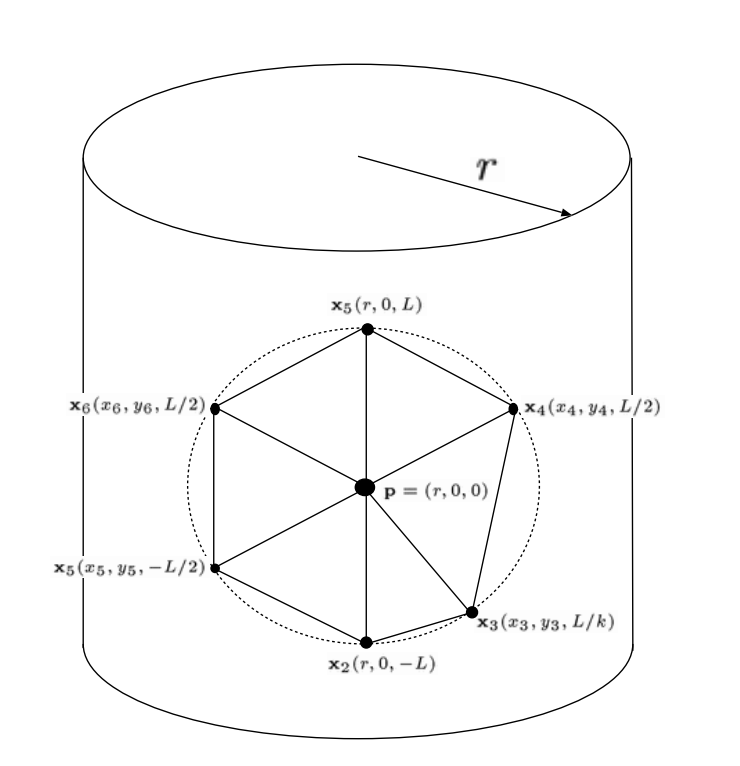
\includegraphics[width = 0.8\textwidth]{2.png}
\end{figure}

Используя формулы выше, можно уменьшить $L$, оставляя $r$ фиксированным, чтобы уменьшить размер шестиугольника. Если шестиугольник меньше, его вершины все еще находятся на цилиндре, качство треугольников сильно не меняется и вершниы становятся более копланарными.
\\
\\
Таким образом, можно оценить сходимость любого метода, уменьшая $L$. Возьмем $r = 2.0$. Результаты представлены в таблице. 
\begin{figure}[H]
	\centering
	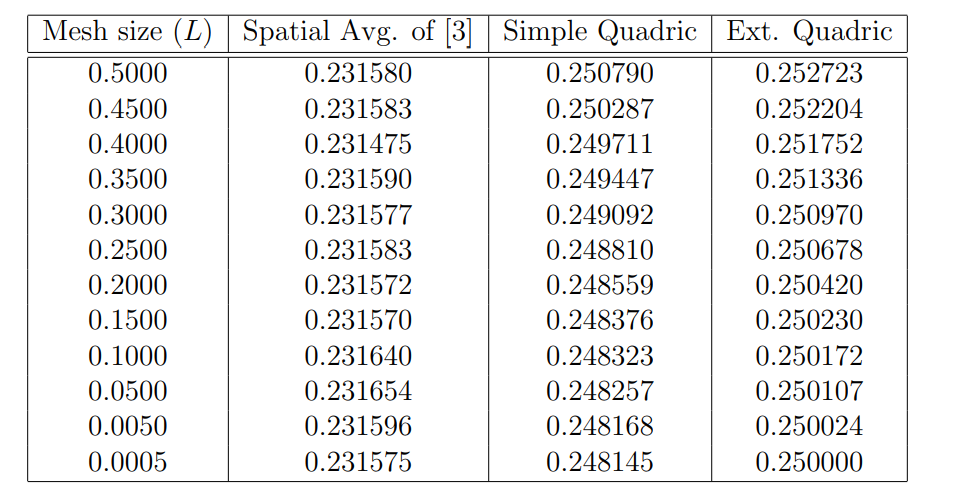
\includegraphics[width = 0.8\textwidth]{3.png}
\end{figure}
Видно, что метод пространственного усреднения имеет конечную ошибку, но не сходится. Даже больше, эта ошибка максимальна среди всех использованных методов. Метод подгонки простыми квадриками сходится к неправильному значению с незначительной ошибкой. Последний же метод показывает лучший результат, он сходится к правильному значению.

\subsection*{Результаты на общих сетках}
\noindent\rule{\textwidth}{1pt}
Модифицированные методы были использованы на нескольких сложных неструктурированных сетках, показав хорошие результаты. Приведем рисунки, отражающие полученные результаты на общих сетках.
\begin{figure}[H]
	\centering
	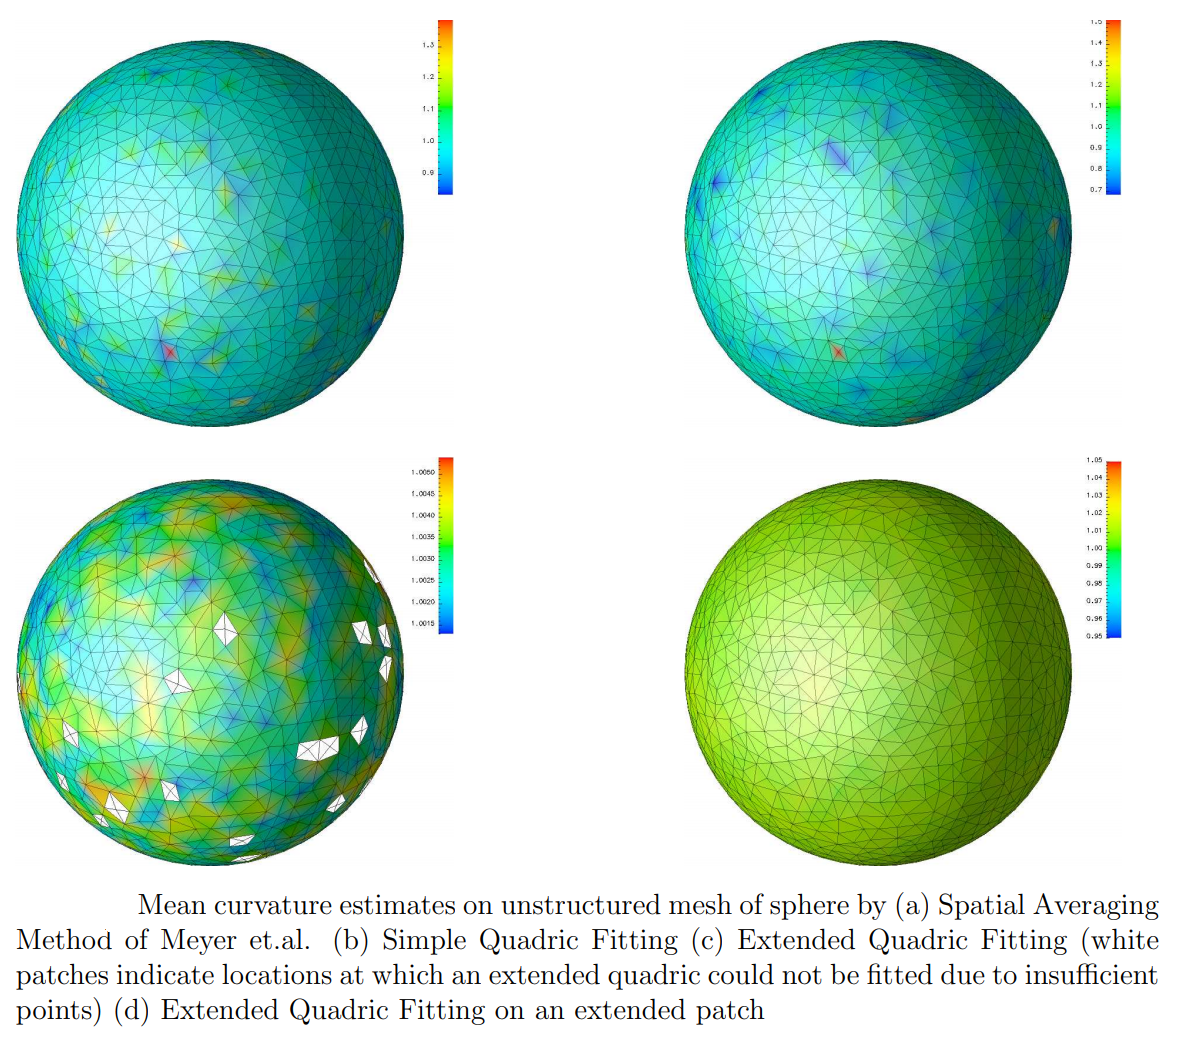
\includegraphics[width = 0.8\textwidth]{4.png}
\end{figure}
\begin{figure}[H]
	\centering
	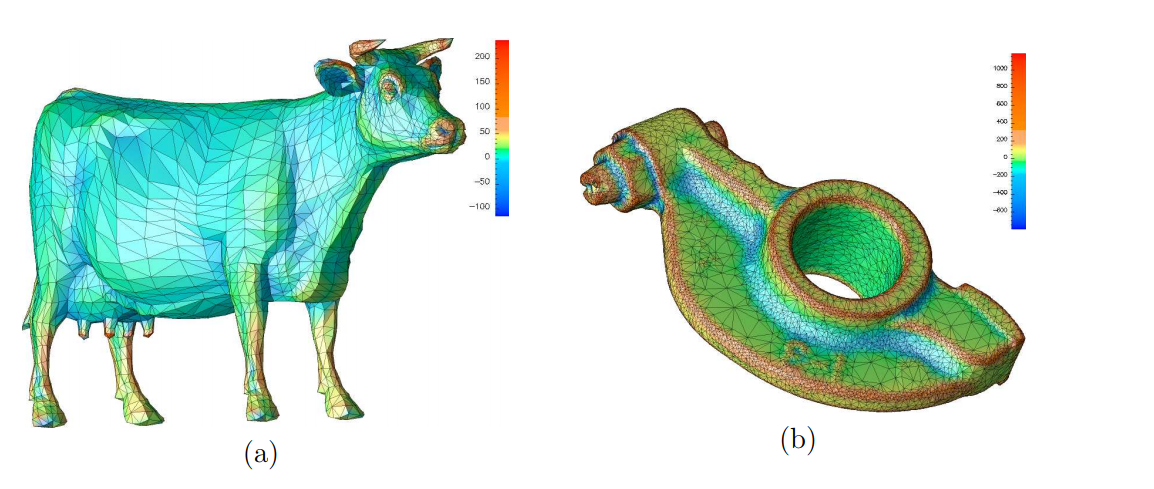
\includegraphics[width = 0.8\textwidth]{5.png}
\end{figure}

\subsection*{Результаты и обсуждения}
\noindent\rule{\textwidth}{1pt}
В данной работе были предложены некоторые оценочные методы для кривизны для неструктурированных сеток. Заключено, что расширенный метод приближения квадриков с некоторым расширением считается автором наиболее точным.

\subsection*{Ссылки и литература}
\noindent\rule{\textwidth}{1pt}
Вся информация взята из единого источника Rao V. Garimella, Blair K.Swartz "Curvature Estimation for Unstructured Triangulations of Surfaces" October 17, 2003 и является лишь переводом с английского языка на русский для курсовой работы. Автор данного перевода не считается контрибьютером в изначальную работу и не берет на себя никаких обязательств.

\end{document}